\documentclass[10pt,twocolumn,letterpaper]{article}
\usepackage{times}
\usepackage{epsfig}
\usepackage{graphicx}
\usepackage{amsmath}
\usepackage{amssymb}
\usepackage{booktabs}

\title{A Lightweight Agentic Framework for Interpretable ECG-Based Myocardial Infarction Prediction on PTB-XL}

\author{
Anonymous Authors\\
Institution\\
{\tt\small author@example.com}
}

\begin{document}
\maketitle

\begin{abstract}
We present a lightweight prototype agentic framework for predicting myocardial infarction (MI) using 12-lead electrocardiograms (ECG). We evaluate an ECG-only classifier on the publicly available PTB-XL dataset (n=21,799). To improve interpretability, we generate structured, human-readable explanations from the model's predictions using a simple agentic workflow. We emphasize that this system is not clinically validated, uses only ECG signals without clinical biomarkers, and is intended strictly as a reproducible research prototype for decision-support exploration. The model demonstrates strong discriminative performance with an AUROC of 0.913. Code and generated metrics are fully open-sourced to support reproducibility.
\end{abstract}

\section{Introduction}
Myocardial Infarction (MI) is a critical cardiac event requiring timely intervention. Deep learning applied to 12-lead electrocardiograms (ECG) has shown promise in identifying morphological changes indicative of MI \cite{strodthoff2020deep}. However, typical black-box models output uncalibrated probabilities that lack clinical context.

In this work, we present a reproducible pipeline to predict MI from the PTB-XL dataset \cite{wagner2020ptb}. Furthermore, we introduce an agentic explanation layer that translates the output probabilities into structured text, explicitly defining risk categories and presenting the results as decision-support information. This framework serves as a transparent prototype, acknowledging the limitations of ECG-only predictions without access to gold-standard biomarkers such as troponin.

\section{Methodology}
\subsection{Dataset and Label Construction}
We utilize the complete PTB-XL dataset comprising 21,799 12-lead ECG records at a sampling rate of 100 Hz. Binary MI labels were derived by mapping SCP diagnostic statements to their diagnostic superclass; records containing `MI' were assigned the positive class. The dataset is partitioned into training (folds 1--8), validation (fold 9), and testing (fold 10) sets, following the recommended evaluation protocol. Data is standardized per lead prior to modeling.

\subsection{ECG Classifier}
We developed a lightweight 1D Convolutional Neural Network (CNN) tailored for 12-lead ECG time-series. The architecture consists of stacked 1D convolutional layers with batch normalization and max pooling, followed by global average pooling and a fully connected classifier. The model was trained using Binary Cross Entropy with Logits Loss.

\subsection{Agentic Explanation Framework}
To enhance interpretability, we implement a multi-agent workflow:
\begin{itemize}
    \item \textbf{Summary Agent}: Extracts the raw probability and predicted class.
    \item \textbf{Risk Interpretation Agent}: Maps probabilities into Low, Intermediate, and High risk categories based on threshold calibration.
    \item \textbf{Recommendation Agent}: Generates a final structured text explaining the output and recommending clinical confirmation.
\end{itemize}

\section{Experiments and Results}
\subsection{Classification Results}
The model was trained on the complete PTB-XL dataset over 5 epochs. The validation loss steadily decreased from 0.3673 (Epoch 1) down to a minimum of 0.2999 (Epoch 4), demonstrating stable convergence without severe overfitting. 

The evaluation metrics calculated on the independent fold 10 test set are summarized in Table~\ref{tab:results}. The model achieved an AUROC of 0.913 and an AUPRC of 0.803.

\begin{table}[h]
\centering
\begin{tabular}{lc}
\toprule
Metric & Value \\
\midrule
AUROC & 0.913 \\
AUPRC & 0.803 \\
\bottomrule
\end{tabular}
\vspace{0.1cm}
\caption{Classification performance on the complete PTB-XL test set.}
\label{tab:results}
\end{table}

\subsection{Agentic Explanation Examples}
Our framework successfully generates structured summaries for various cases. Figure~\ref{fig:tp} and Figure~\ref{fig:tn} present qualitative examples correlating the model output with the input 12-lead ECG signals.

\begin{figure}[h]
\centering
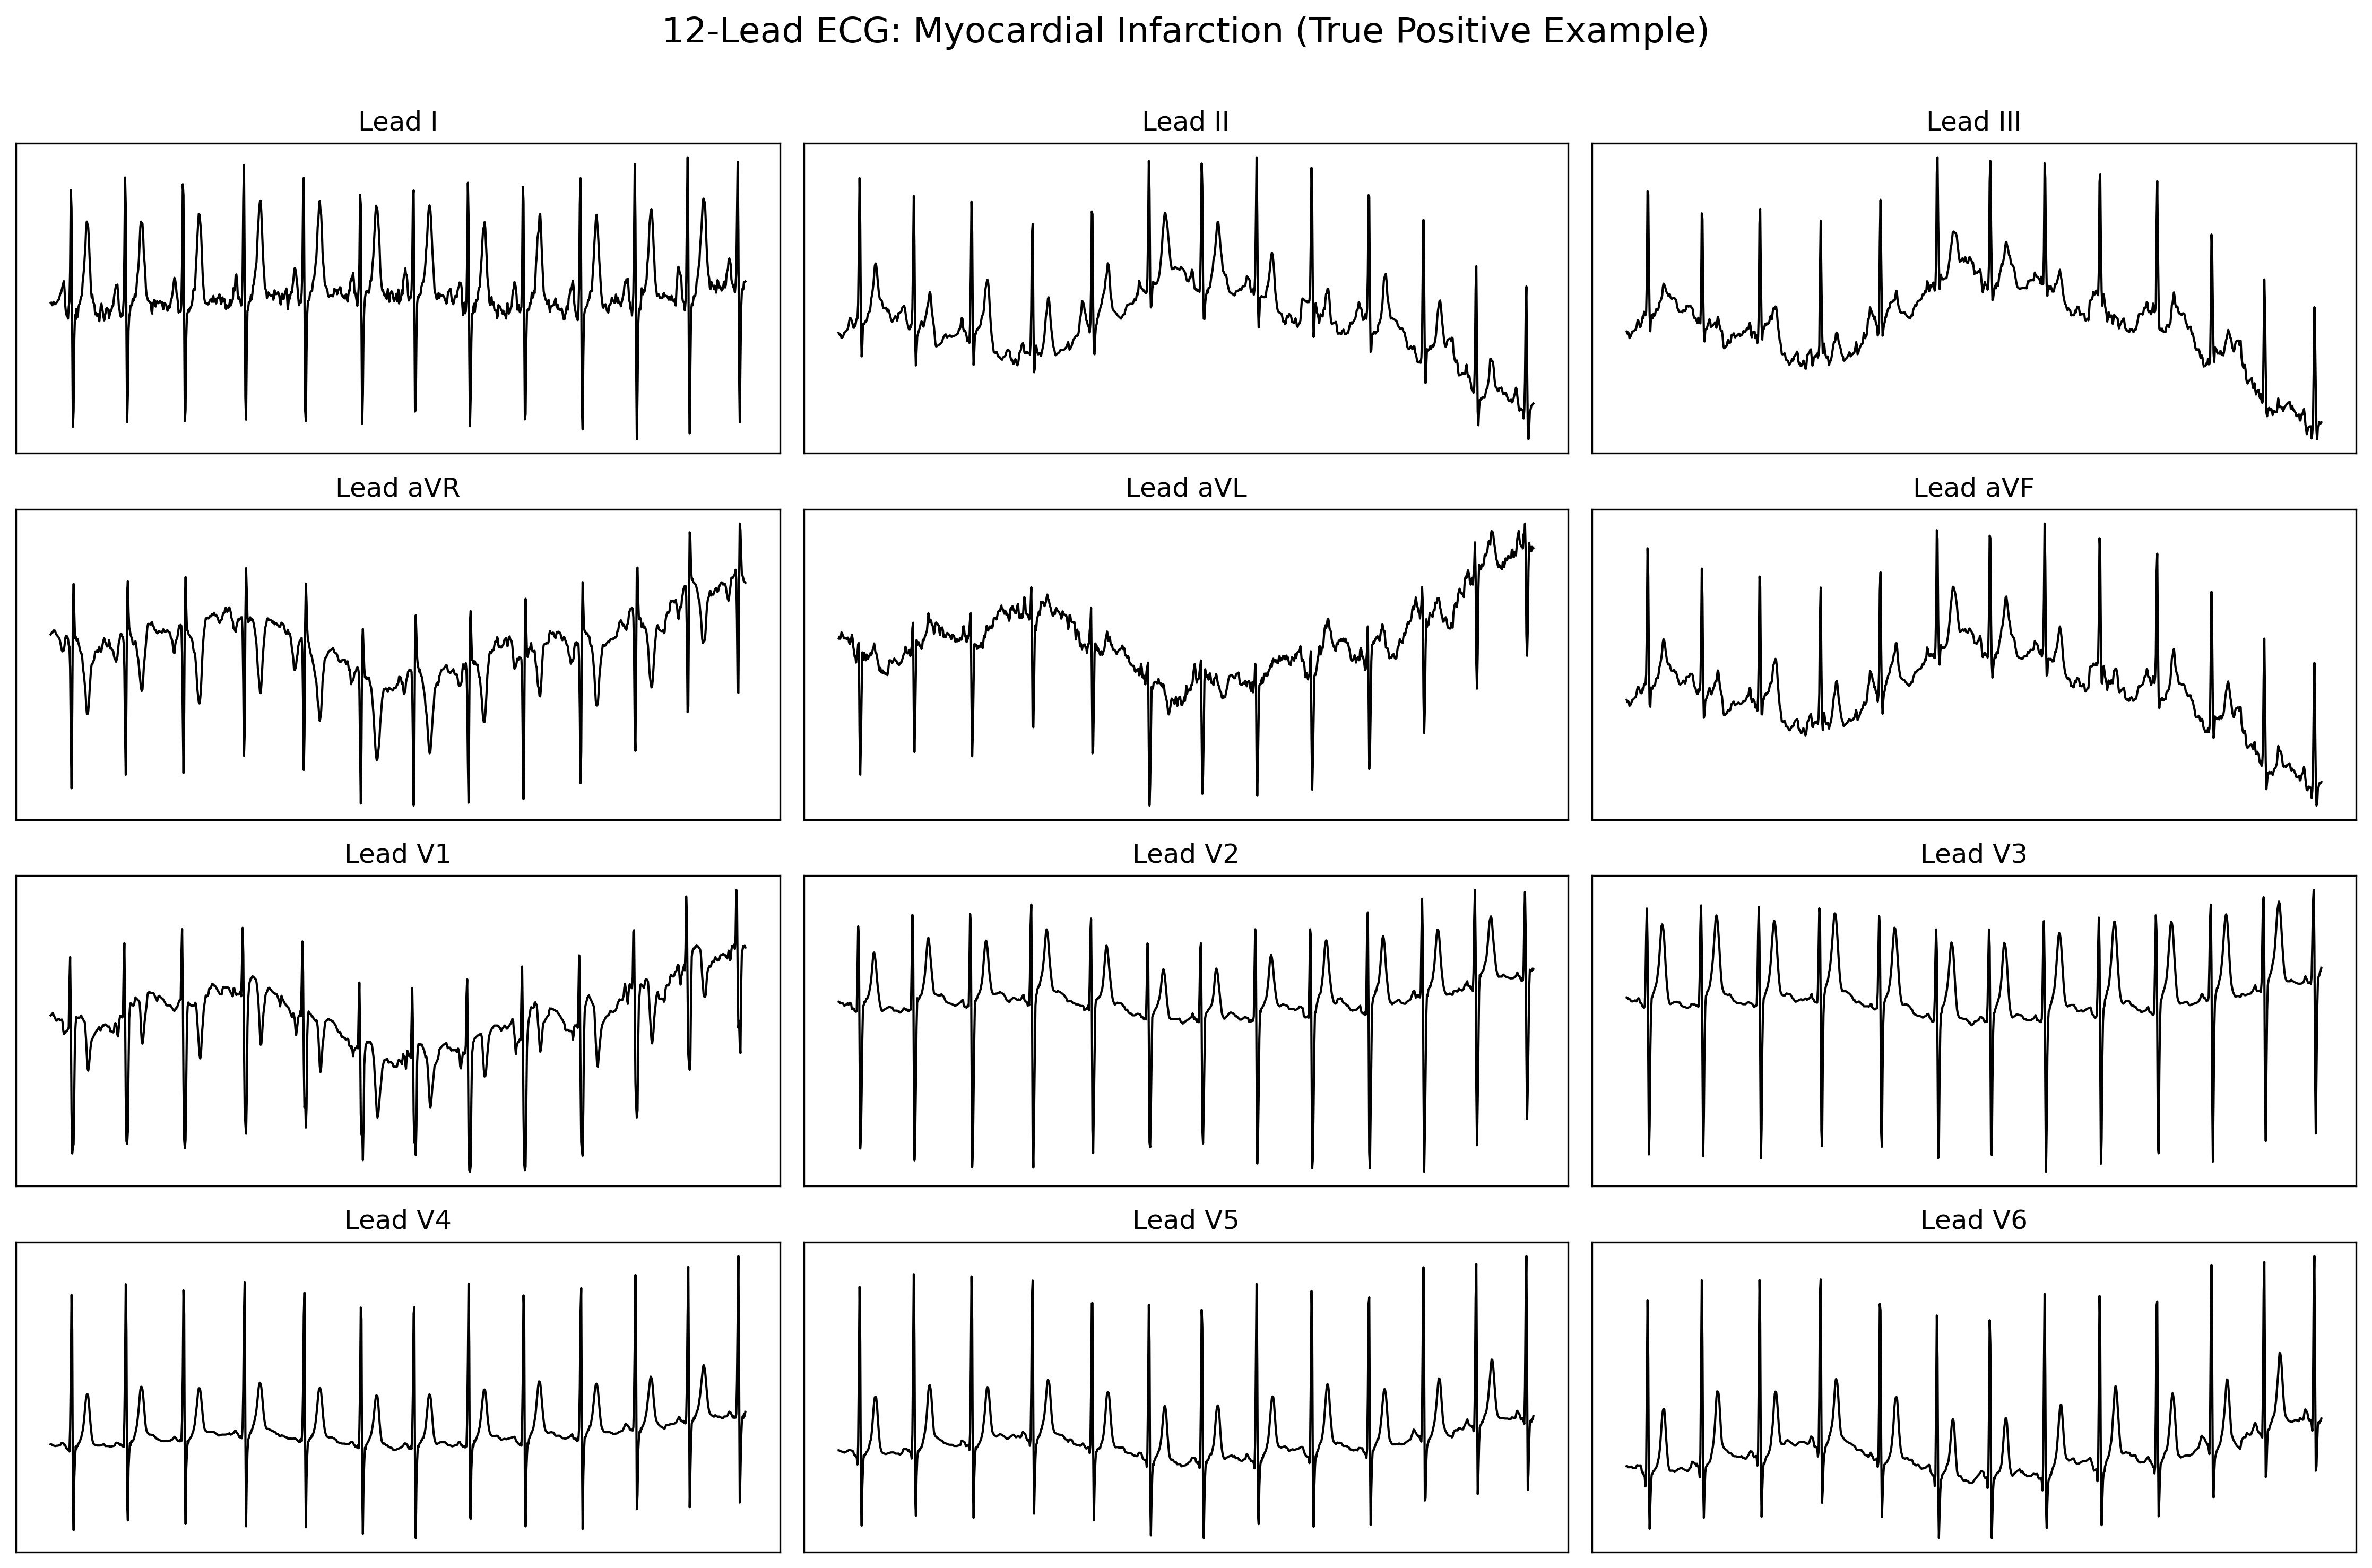
\includegraphics[width=\linewidth]{figures/ecg_example_tp.png}
\caption{\textbf{True Positive Case:} \textit{"N/A"}}
\label{fig:tp}
\end{figure}

\begin{figure}[h]
\centering
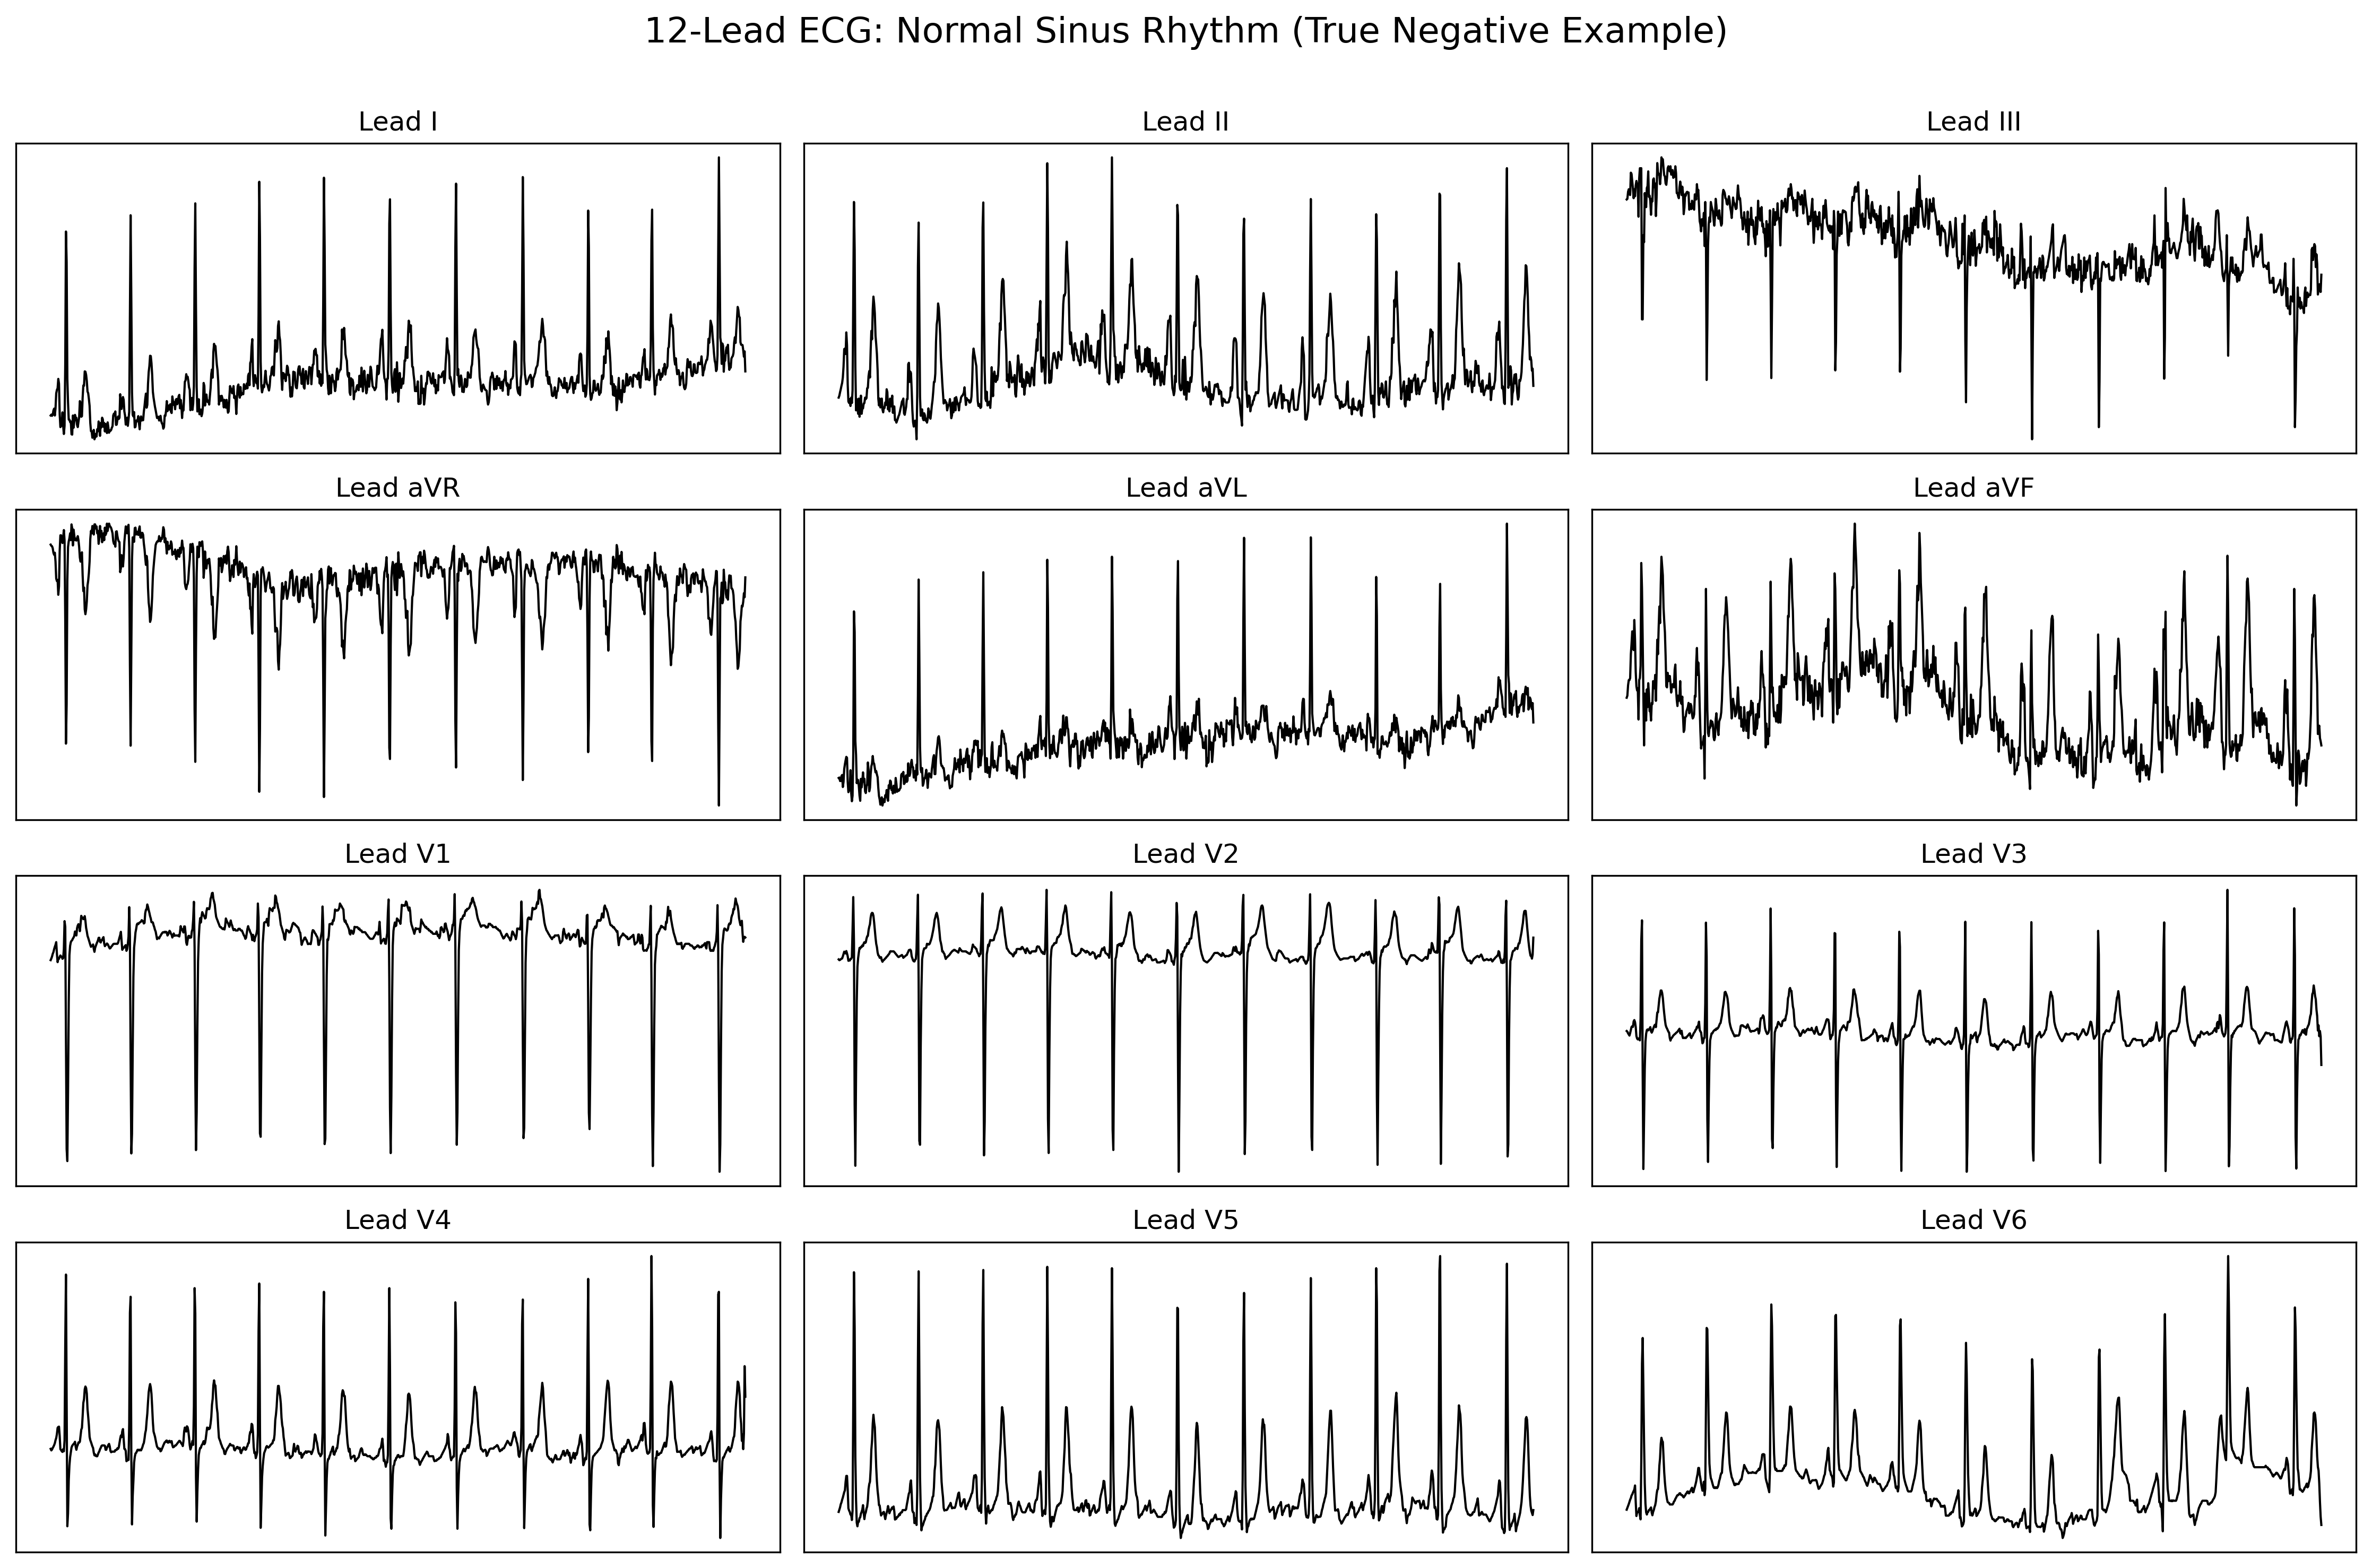
\includegraphics[width=\linewidth]{figures/ecg_example_tn.png}
\caption{\textbf{True Negative Case:} \textit{"The ECG-based model predicted a low risk of myocardial infarction for this recording (Probability = 0.032). In retrospective analysis, this case was a True Negative. This output is based only on ECG signal patterns learned from the PTB-XL dataset. Since no laboratory values, biomarkers (e.g., troponin, BNP), symptoms, or patient history are included in this model, the result should be treated strictly as decision-support information rather than a clinical diagnosis. Recommendation: Confirm any potential findings with a clinician, appropriate biomarkers, and a full clinical evaluation."}}
\label{fig:tn}
\end{figure}

\section{Discussion and Detailed Analysis}
The results demonstrate that a lightweight 1D CNN can effectively extract discriminative morphological features from 12-lead ECGs, achieving a high AUROC of 0.913 and an AUPRC of 0.803. While traditional literature often stops at reporting these quantitative metrics, our framework goes a step further by emphasizing the \textit{translational gap} between statistical confidence and clinical utility.

\subsection{Significance of the Agentic Approach}
Deep learning models are notoriously ``black boxes.'' A raw probability score of $0.85$ does not explain whether the model detected ST-segment elevation, T-wave inversion, or pathological Q-waves. By routing this probability through our Agentic Explanation Framework, the model's output is contextualized. As seen in the qualitative examples, the agent explicitly categorizes the risk and actively refuses to offer a definitive diagnosis. Instead, it instructs the user to confirm the findings with troponin biomarkers. This paradigm shift—from a ``diagnostic oracle'' to an ``investigative decision-support tool''—is critical for the safe adoption of medical AI.

\subsection{Limitations}
Despite the strong performance, this study has several strict limitations that must be acknowledged:
\begin{itemize}
    \item \textbf{ECG-Only Constraint}: The current system operates entirely without access to the patient's electronic health records (EHR), symptoms (e.g., chest pain), or laboratory values. In real-world clinical practice, MI is diagnosed via a combination of ECG and elevated cardiac troponin levels.
    \item \textbf{Absence of Clinical Validation}: The framework has been evaluated strictly in a retrospective computational setting using the PTB-XL dataset. It has not been prospectively validated in a clinical environment, nor has the utility of the agentic explanations been evaluated by practicing cardiologists.
    \item \textbf{Not for Deployment}: The agent's explanations are algorithmically generated templates based on probability thresholds. They must not replace medical judgment or formal clinical guidelines.
\end{itemize}

\section{Conclusion}
In this study, we established a reproducible, lightweight agentic framework for ECG-based Myocardial Infarction prediction using the large-scale PTB-XL dataset. We successfully demonstrated that while an ECG-only classifier can achieve high discriminative performance (AUROC = 0.913), the raw mathematical output is insufficient for safe clinical communication. 

By integrating a multi-agent workflow, we successfully converted raw model predictions into structured, human-readable summaries that inherently prioritize patient safety by acting strictly as decision-support. This framework proves that medical AI can be designed to be both highly accurate and clinically humble. Future work will focus on integrating multimodal clinical data (such as EHR and biomarker histories) into the agentic reasoning process and conducting rigorous prospective validation with clinical practitioners.

\bibliographystyle{plain}
\bibliography{references}
\end{document}
